\chapter{基于物理信息启发的双分支Swin Transformer预测模型的架构设计}
\label{chap:3}

\section{总体架构设计思路}
\label{sec:3-1}
野火蔓延是一个高度复杂的非线性动力学过程，受到气象、地形与植被等多种环境因素的共同影响，并表现出明显的多尺度时空耦合特性。现有深度学习方法大多采用“全变量直接拼接”的方式，将静态与动态特征统一输入模型进行学习。虽然这种方法实现简单，但往往忽略了不同类型变量在时间和物理意义上的差异，尤其难以有效刻画气象因子背后所蕴含的热力学过程与演化规律。

针对上述问题，本章提出一种基于物理启发的时空解耦双分支 Swin Transformer 野火预测模型。该模型从特征属性出发，将静态地理信息与动态气象信息分别建模，通过双分支结构实现时空特征的解耦学习。同时，在动态分支中引入与火灾传播相关的物理先验，以增强模型对环境变化过程的表征能力，在提升预测性能的同时提高结果的可解释性。模型整体框架如图\ref{fig:3-1-pipeline}所示。

时空特征解耦原则主要是由于大气环境因子的演化周期存在本质差异。地形地貌等属于静态空间特征，在短期的预测时间窗口内几乎不变。气象条件则属于动态时空特征，呈现出随时间演变的特征。若统一采用三维网络处理，会导致模型对静态背景进行冗余建模，增加过拟合风险。本架构采用双分支编码策略，均基于Swin Transformer构建，利用二维分支专门提取静态特征，三维分支提取动态气象特征。两条分支独立编码，并在后续利用地理感知交叉注意力机制进行融合，有效提升了模型的计算效率与预测精度。

物理机制引导原则旨在弥补模型缺乏物理先验的缺陷。在数据输入阶段，本研究将气温与露点温度重构为饱和水汽压差（Vapor Pressure Deficit，VPD）。这一预处理规避了神经网络拟合复杂热力学公式的困难，使模型能够直接感知可燃物的水分状态。在特征融合阶段，针对传统注意力机制均匀发散的局限，本架构将风场矢量作为物理偏置注入交叉注意力模块。通过计算风向与空间相对向量的点积，模型能够捕捉更多风向信息，更契合野火随风蔓延的气象动力学规律。

\begin{figure}[htbp]
    \centering
    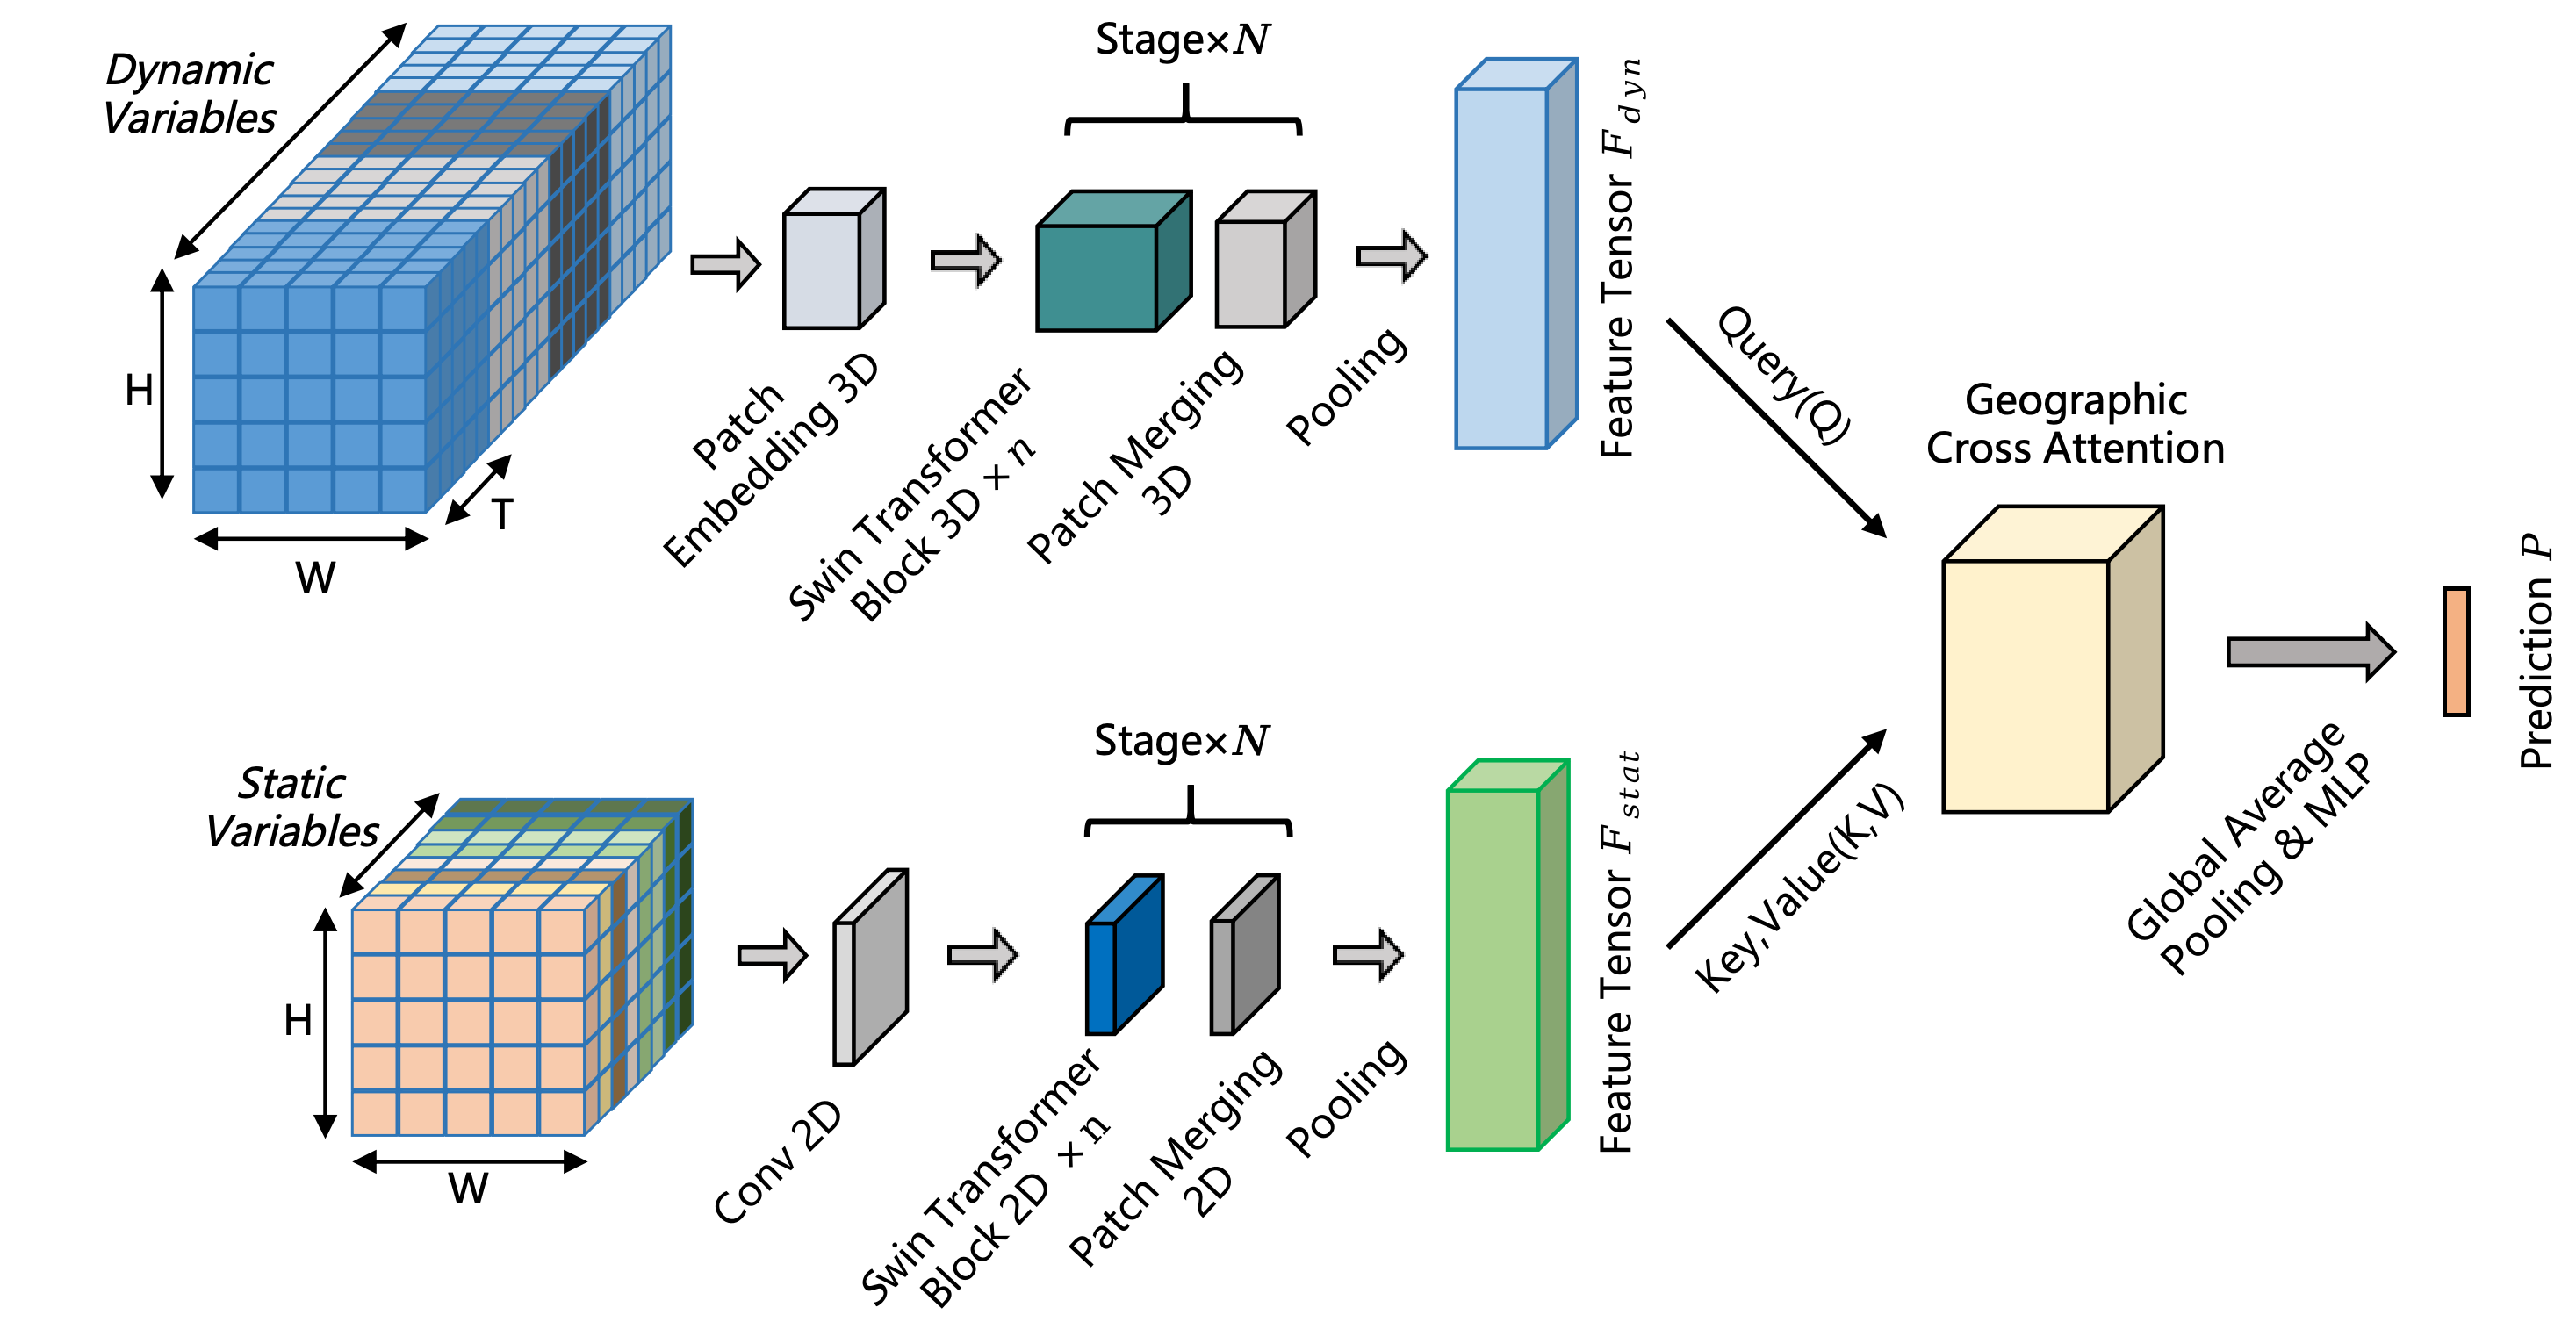
\includegraphics[width=0.9\textwidth]{img/chap3/3-1-pipeline.png}
    \caption{预测模型整体架构设计}
    \label{fig:3-1-pipeline}
\end{figure}

\section{Swin Transformer基础原理}
\label{sec:3-2}
Swin Transformer架构由微软亚洲研究院在2021年提出\cite{liu2021swin}。在计算机视觉领域，卷积神经网络（CNN）长期占据主导地位。然而，受自然语言处理（NLP）领域 Transformer\cite{vaswani2017attention} 架构巨大成功的启发，研究者开始探索如何利用其核心的自注意力机制（Self-attention）来建模数据中的长程依赖关系。Vision Transformer（ViT）是将 Transformer 直接应用于视觉任务的先驱工作\cite{dosovitskiy2020image}。它通过将图像划分为固定大小的斑块（Patches），并将每个patch视为一个token输入到Transformer 编码器，证明了在超大规模数据集预训练下，Transformer 能够达到甚至超越 CNN 的性能。然而，ViT 在作为通用骨干网络时面临两大核心挑战，一是尺度不适配，ViT 生成的是单分辨率的低分辨率特征图，难以应对视觉图像尺度变化剧烈的任务；二是计算复杂度过高，ViT 的自注意力计算是在全局范围进行的，其计算复杂度与图像尺寸成平方级增长（O${(hw)}^2$），这使得处理高分辨率图像变得异常昂贵。

为了解决上述问题，\textcite{liu2021swin}提出了 Swin Transformer，它能够作为一种新的视觉Transformer，成为计算机视觉领域的通用骨架。Swin Transformer是一个分层的Transformer，输入的特征通过滑动窗口（\textbf{S}hifted \textbf{Win}dows）来计算。滑动窗口的方案将自注意力（Self-Attention）计算局限于不重叠的局部窗口，同时允许跨窗口连接，从而提高了效率。这种分层架构具有在不同尺度建模的灵活性，并且相对于图像大小具有线性计算复杂度。

图\ref{fig:3-2-swintransformer}展示了Swin Transformer的整体架构，Swin Transformer的参数可以调整，图中所示为\cite{liu2021swin}中提及的参数量最小的版本，Swin-T（C = 96, layer numbers = {2, 2, 6, 2}）。对于一张RGB图像的输入，如图\ref{fig:3-2-swintransformer}(a)所示，Swin Transformer首先通过像ViT一样的切片（Patch Splitting）模块将输入RGB图像拆分为不重叠的Patch。每个Patch都被视为一个token，其特征被设置为原始像素RGB值的拼接。若使用的Patch大小为$4\times 4$，则每个Patch的特征维数为$4\times 4\times 3=48$。在该原始值特征上施加线性嵌入层（Embedding），将其投影到任意维度（记为C）。

\begin{figure}[htbp]
    \centering
    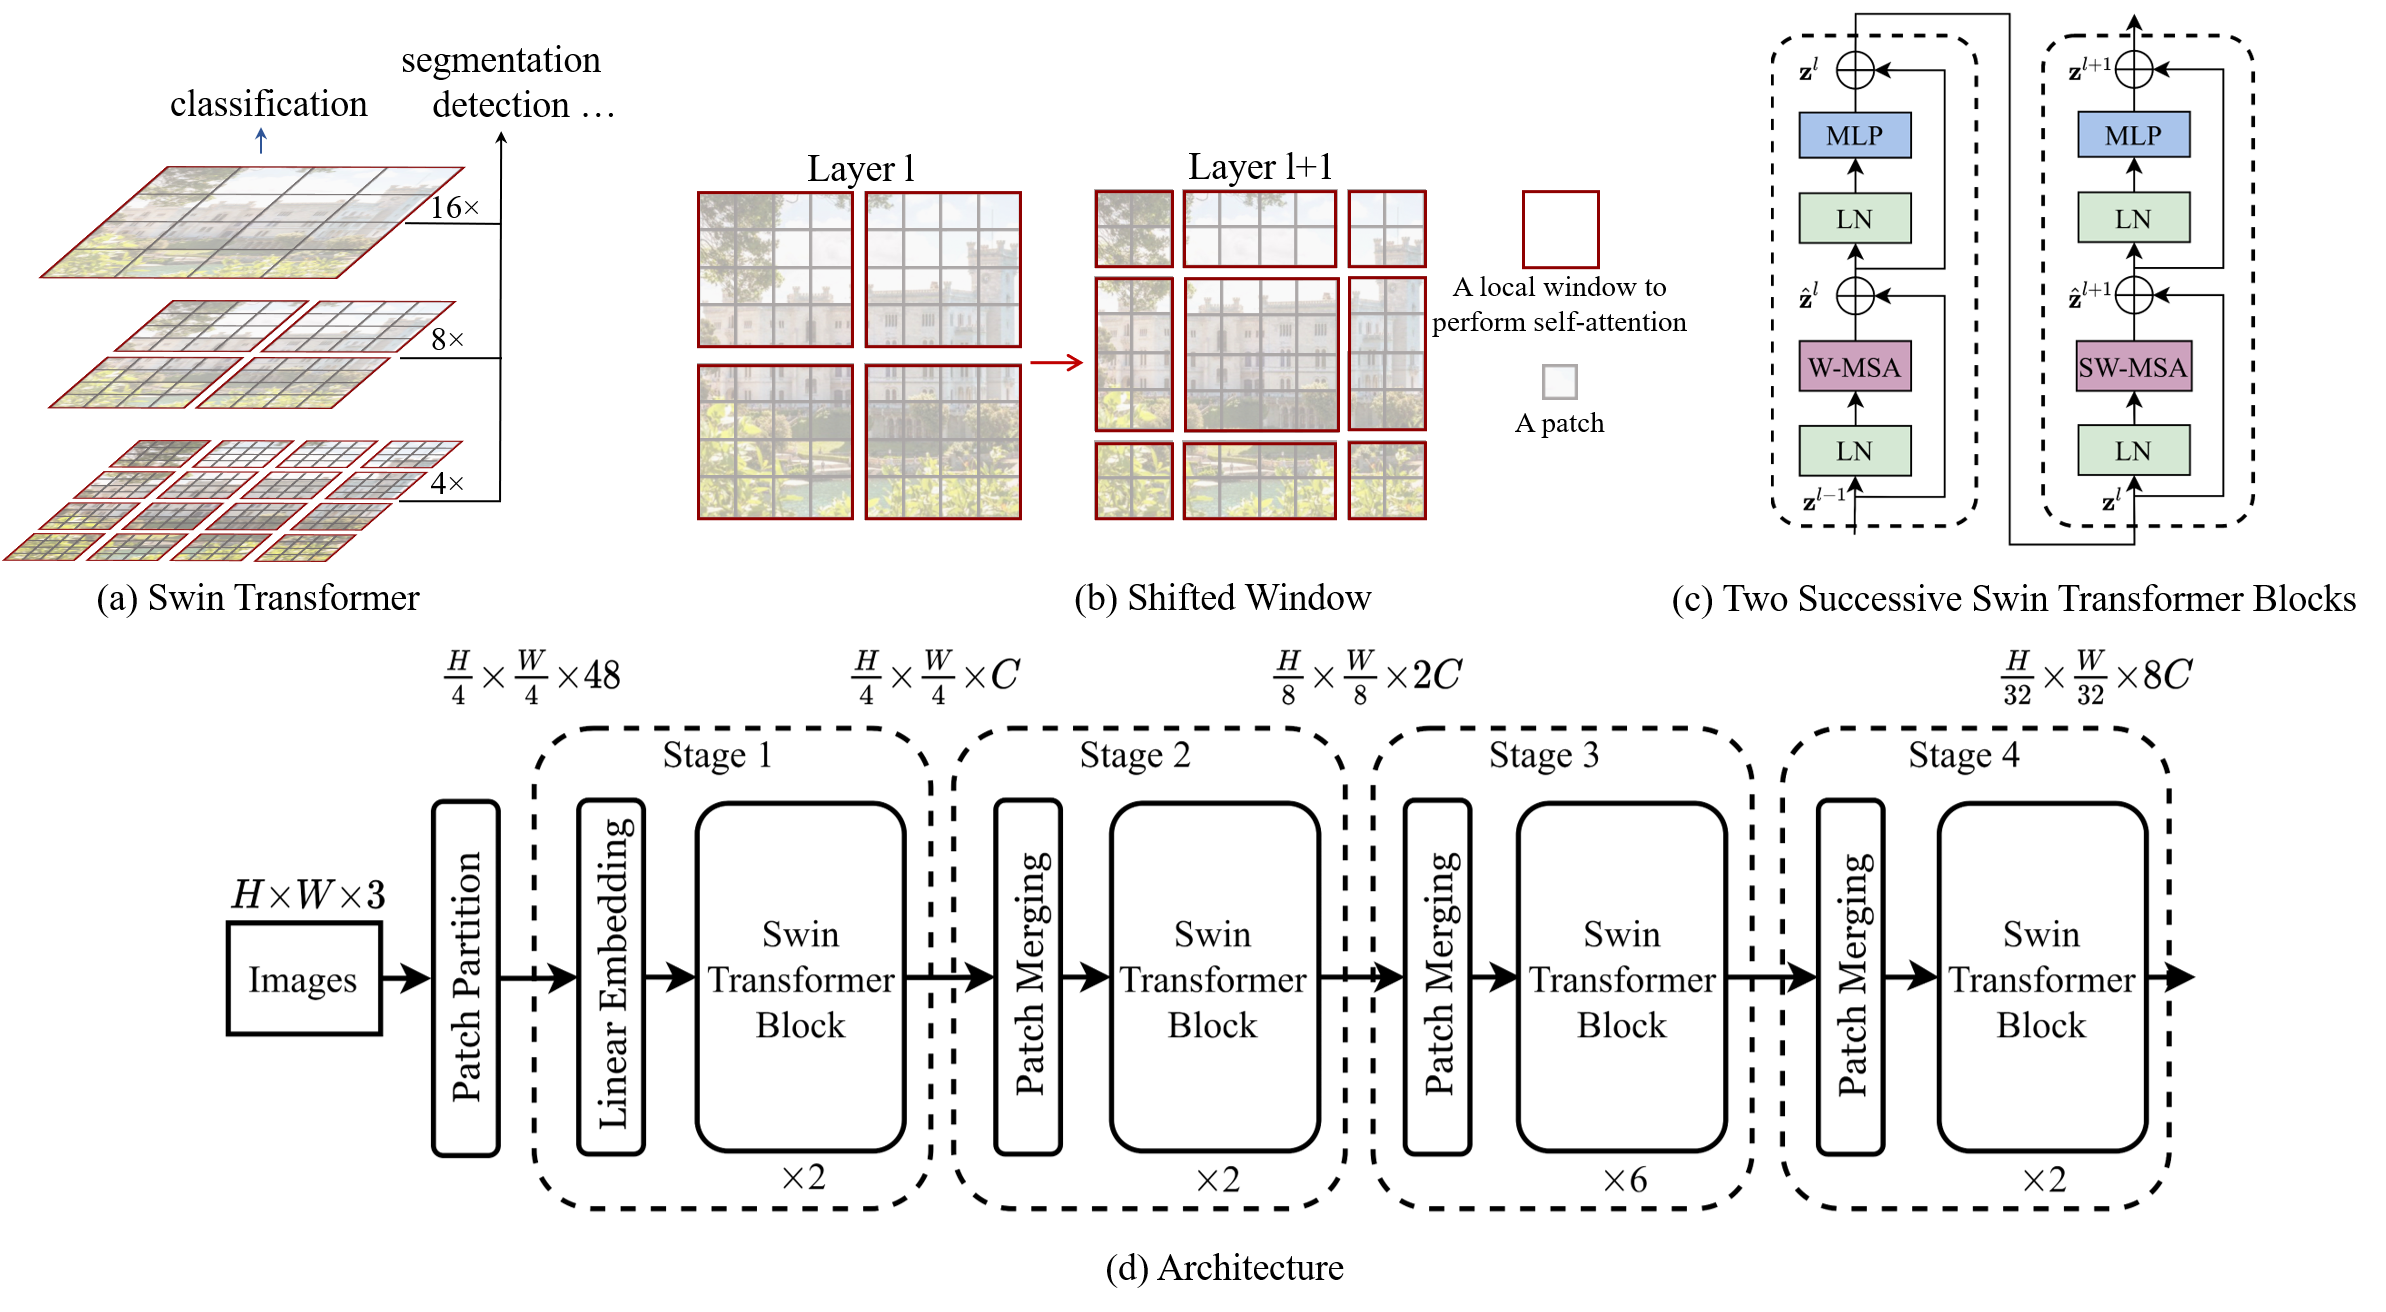
\includegraphics[width=0.9\textwidth]{img/chap3/3-2-swintransformer.png}
    \caption{Swin Transformer结构图，引用自\cite{liu2021swin}}
    \label{fig:3-2-swintransformer}
\end{figure}

如\ref{fig:3-2-swintransformer}(d)中所示，原始图像经过Patch切分后需要经过4个Stage，得到最终输出的预测值。第一个Stage由Linear Embedding和2个Swin Transformer Block组成，其余的Stage均由Patch Merging和数个Swin Transformer组成。这即是生成层次化的特征表示的过程，随着网络深度的增加，Token的数量通过斑块合并层（patch merging layers）逐渐减少，具体而言，从$\frac{H}{4}\times \frac{W}{4}\times 48$到$\frac{H}{4}\times \frac{W}{4}\times C$最终到$\frac{H}{32}\times \frac{W}{32}\times 8C$，最终实现了从整张图片中提取低维度特征的效果。对于我们的野火风险预测任务，虽然输入的不是RGB图像，而是静态变量或动态变量的组合，但原理与处理方法与之相似。

Swin Transformer Block的构建方式是将标准 Transformer 模块中的全局多头自注意力（Multi-head Self-Attetion，MSA）模块替换为基于移动窗口机制的注意力模块，同时保持其余网络层结构不变。相关架构如图\ref{fig:3-2-swintransformer}(c)所示，单个 Swin Transformer 模块包含一个基于移动窗口的多头自注意力模块，以及紧随其后的两层多层感知机（MLP），该感知机内部采用 GELU 非线性激活函数。此外，在每个自注意力模块和多层感知机之前均应用了层归一化（LN）操作，并在每个模块的输出端都加入了残差连接。

下面我们详细介绍基于移动窗口的多头自注意力模块，也是Swin Transformer架构的核心创新之处。

标准的Transformer架构及ViT\cite{dosovitskiy2020image}都进行全局自注意力计算，即计算一个token与其他所有token之间的关系，导致参数数量的二次复杂度，因此不适合需要大量token以实现密集预测或高分辨率图像的问题。为了高效建模，Swin Transformer在局部窗口内计算自注意力的值，这些窗口由图像均匀分割且不重叠。假设每个窗口包含$h\times w$个Patch，每个Patch的形状为$M\times M$，则全局MSA模块和基于窗口的MSA模块（W-MSA）的计算复杂度分别为：
\begin{equation}
    \Omega_{\text{MSA}} = 4hwC^2 + 2(hw)^2cm
\end{equation}
\begin{equation}
    \Omega_{\text{W-MSA}} = 4hwC^2 + 2M^2hwC
\end{equation}
其中前者是切片数量$hw$的二次方，而后者在M固定时的计算复杂度是线性的。

窗口的切分（window partitioning）减少了计算复杂度，但限制了不同窗口之间的连接。因此，作者提出了滑动窗口（Shifted window）多头自注意力机制，并在Swin Transformer Block中连续使用交替使用两种划分配置，即W-MSA和SW-MSA。如图\ref{fig:3-2-swintransformer}(b)所示，第一个模块采用了从左上像素开始的常规窗口划分策略，$8\times 8$的特征映射被均匀划分为$2\times 2$个窗口，窗口大小为$4\times 4(M = 4)$。接着，通过将窗口从原始位置向右下方移位$(\lfloor \frac{M}{2}\rfloor,\lfloor \frac{M}{2}\rfloor)$像素，下一模块采用了滑动窗口配置，保证了不同窗口之间信息的连接。采用滑动窗口划分方法，连续的Swin Transformer Block的计算如下：
\begin{equation}
\begin{aligned}
\hat{\mathbf{z}}^l &= \text{W-MSA}\left(\text{LN}\left(\mathbf{z}^{l-1}\right)\right) + \mathbf{z}^{l-1}, \\
\mathbf{z}^l &= \text{MLP}\left(\text{LN}\left(\hat{\mathbf{z}}^l\right)\right) + \hat{\mathbf{z}}^l, \\
\hat{\mathbf{z}}^{l+1} &= \text{SW-MSA}\left(\text{LN}\left(\mathbf{z}^l\right)\right) + \mathbf{z}^l, \\
\mathbf{z}^{l+1} &= \text{MLP}\left(\text{LN}\left(\hat{\mathbf{z}}^{l+1}\right)\right) + \hat{\mathbf{z}}^{l+1},
\end{aligned}
\end{equation}
其中$\hat{\mathbf{z}}^l$和$\mathbf{z}^l$分别表示块（Block）$l$的 （S）W-MSA 模块和 MLP 模块的输出特征。

此外，移动窗口划分机制存在一个固有缺陷，在移动配置下参与批处理的窗口总数可能会增加，且当窗口滑动时边界处会产生部分尺寸小于$M\times M$的残缺窗口。一种常规的解决方案是将这些残缺窗口零填充（pad）至标准的$M\times M$尺寸，并在计算注意力时将填充区域利用掩码（mask）剔除。然而，当常规划分下的窗口总数较少时（例如仅有$2\times 2$个窗口），这种零填充方案所带来的额外计算开销是较大的（窗口数由$2\times 2$增至$3\times 3$，计算量暴增 2.25 倍）。为此，作者提出了一种更为高效的批处理计算方法，即向左上角方向进行循环移位（cyclic-shifting)，如图\ref{fig:3-2-shifted-window}所示。经过循环移位后，一个完整的批处理窗口可能由多个在原始特征图上不相邻的子窗口拼凑而成。因此，模型引入了掩码机制（masking mechanism），以严格限制自注意力的计算仅在各个原本相邻的子窗口内部进行，保障了计算的高效性。
\begin{figure}[htbp]
    \centering
    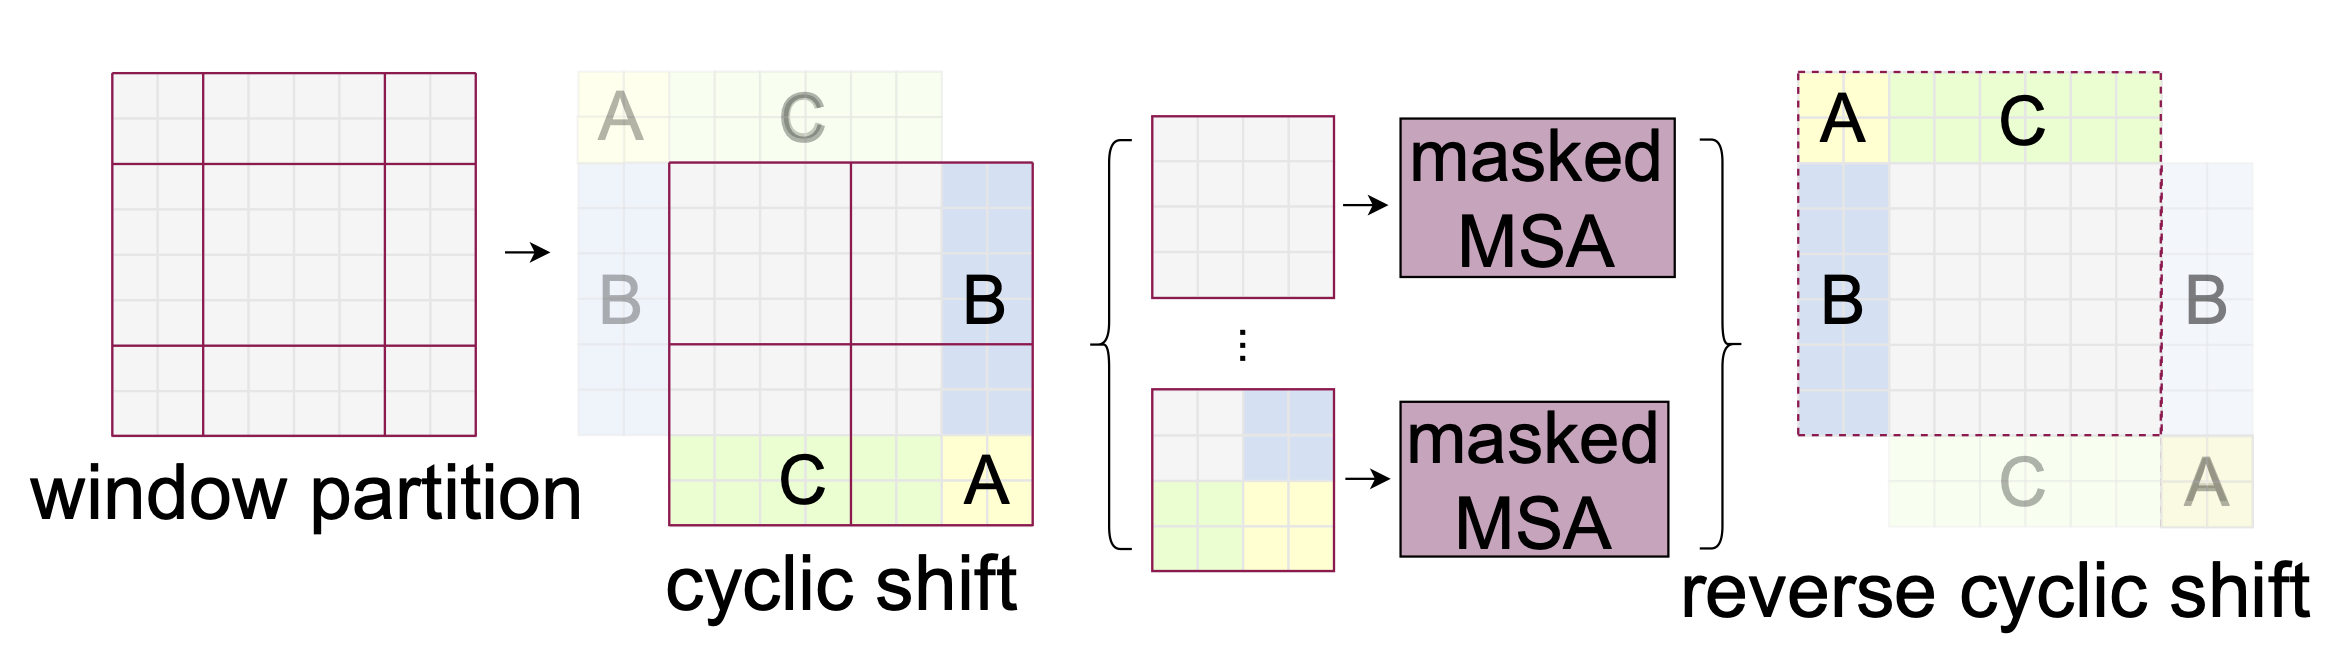
\includegraphics[width=0.9\textwidth]{img/chap3/3-2-shifted-window.png}
    \caption{移位窗口划分中高效批量计算方法的示例，引用自\cite{liu2021swin}}
    \label{fig:3-2-shifted-window}
\end{figure}
在计算自注意力时，作者未使用原始Transformer中的绝对位置编码，而是为每个头（head）引入一个相对位置偏置 $B \in \mathbb{R}^{M^2 \times M^2}$：
\begin{equation}
\text{Attention}(Q, K, V) = \text{SoftMax}(QK^T / \sqrt{d} + B)V,
\end{equation}
其中 $Q, K, V \in \mathbb{R}^{M^2 \times d}$ 分别代表查询（query）、键（key）和值（value）矩阵；$d$ 是查询矩阵和键矩阵的维度，而 $M^2$ 是单个窗口内包含的切片（patch）数量。由于沿每个坐标轴的相对位置均落在 $[-M + 1, M - 1]$ 的区间范围内，作者参数化了一个尺寸较小的偏置矩阵 $\hat{B} \in \mathbb{R}^{(2M-1) \times (2M-1)}$，而矩阵 $B$ 中的取值均直接映射自 $\hat{B}$。

\section{双分支Swin Transformer预测模型}
\label{sec:3-3}
本节主要介绍双分支特征提取网络的具体结构。在\ref{sec:3-2}节对Swin Tranformer基本原理的介绍中，我们知道其在计算机视觉尤其是图像领域有着很好的应用，而野火时空预测任务中的静态变量与动态变量组成的网格和图像的特征有异曲同工之处，因此本研究选择基于Swin Transformer搭建预测模型。为了让它能够处理野火预测任务中复杂的气象和地理数据，我们将模型拆分成了两个并行的分支：一个 3D 分支用于动态变量，另一个 2D 分支处理静态变量。

两条分支都保留了 Swin Transformer 最核心的滑动窗口注意力机制（Shifted Window Attention）和逐步下采样（Patch Merging）的结构。但为了适配具体的输入数据，我们对网络的层数、通道数和窗口大小进行了重新设置。
\subsection{气象动力学特征提取模块：Swin Transformer 3D}
\label{sec:3-3-1}

该模块负责对多变量动态气象序列进行时空联合编码。模型的输入为动态气象张量 $X_{dyn} \in \mathbb{R}^{B \times C_{in} \times D \times H \times W}$，其中批次大小为 $B$，特征通道数 $C_{in}=10$（即输入十个动态变量），时间序列长度 $D=10$，空间分辨率 $H=W=25$。

由于在本任务中输入的时空变量为三维变量，每个的特征维度为 $[10,25,25]$，共有 10 个动态变量，因此普通的 Swin Transformer 架构无法直接处理动态变量。本研究采用 Swin Transformer3D \cite{yang2025swin3d}，其与 \ref{sec:3-2} 节中介绍的基本原理类似，但将自注意力机制的作用域从二维平面拓展至了三维时空域。在常规的二维架构中，模型仅能在单一时间断面的空间窗口内捕捉静态分布，无法跨越时间步感知气象变量的物理演化。Swin Transformer 3D 的核心原理在于引入了3D Swin Transformer Block，使用三维局部窗口与三维循环移位（3D Cyclic-shifting）机制。

如图\ref{fig:3-3-swin3d}所示，模型将输入的时空张量划分为多个大小为 $(P, M, M)$ 的非重叠时空立方体，并在这些独立的三维窗口内计算自注意力。随后，网络在时间、高度和宽度三个维度上同步施加尺寸为 $(\lfloor P/2 \rfloor, \lfloor M/2 \rfloor, \lfloor M/2 \rfloor)$ 的空间错位，并结合三维掩码（Mask）机制，使得前一网络层中被物理截断的时序片段在深层网络中得以重新拼接。Swin Transformer3D提出后，被广泛应用于视频、三维体素等领域，并具有很好的效果。这一机制打破了原有结构难以处理含时变量的局限，赋予了模型强大的时域感受野，使其能够精准捕获变量的时空特征。

\begin{figure}[htbp]
    \centering
    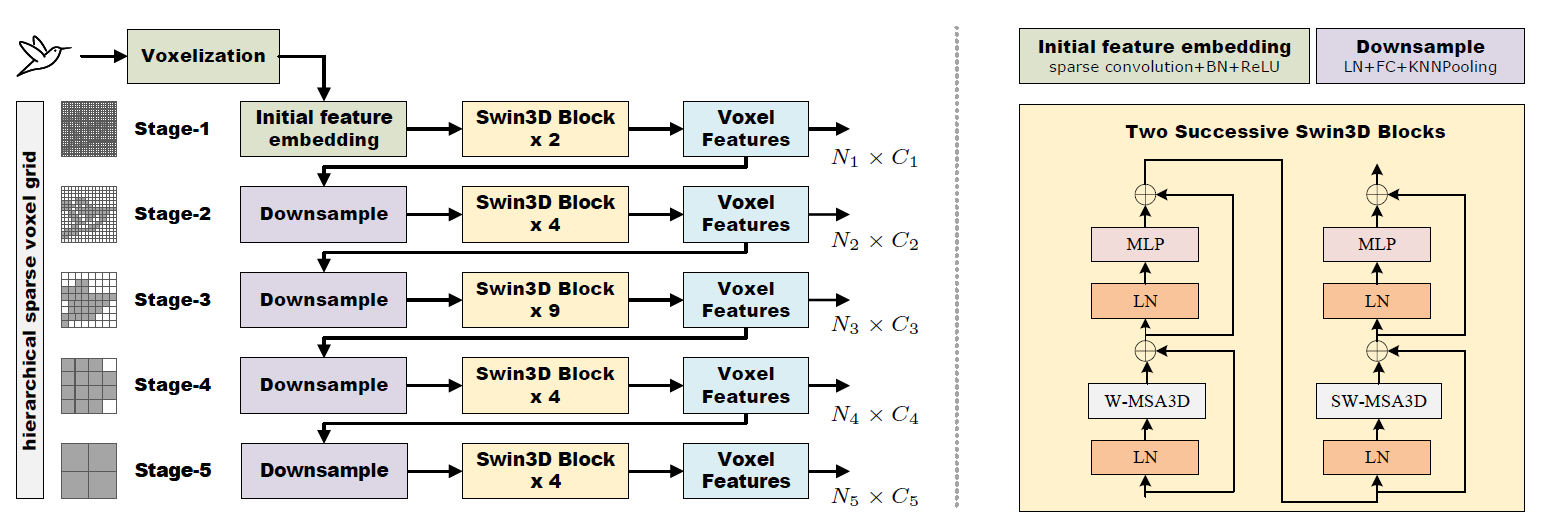
\includegraphics[width=0.9\textwidth]{img/chap3/3-3-swin3d.png}
    \caption{Swin Transformer 3D结构图，引用自\cite{yang2025swin3d}}
    \label{fig:3-3-swin3d}
\end{figure}

针对本研究所使用的小尺度野火气象数据集，本模块对标准的三维架构进行了参数适配。首先，在特征嵌入（Patch Embedding）阶段，模型利用核大小与步长均为 $(1, 1, 1)$ 的三维卷积，将跨越 10 个动态变量跨通道融合并映射至 $C=32$ 的高维特征空间。其次，在注意力窗口尺寸的设定上，模型采用了 $\mathcal{W}_{dyn}=(3, 5, 5)$ 配置。空间窗口尺寸设置为5，因为能够被输入空间边长 25 严格整除；时间窗口尺寸设置为2，也能够被时间长度10整除，意味着模型在单层前向传播中综合计算相邻2日天气波动，并能够在不同窗口之间进行连接。同时，这种设置从底层逻辑上消除了边缘零填充（Padding）所引发的边界噪声与算力消耗。

网络主体构建了包含三个阶段（Stage）的时空特征提取层，各阶段的Swin Transformer Block深度配置为 $[2, 2, 8]$，并在经过多尺度下采样后，输出维度为 $\mathbb{R}^{B \times C_{out} \times D_{out} \times H_{out} \times W_{out}}$ 的高维张量。在输出端，模块沿时间维度 $D_{out}$ 执行均值聚合（Mean Pooling）操作，将三维时空表征为二维空间特征图，从而在保留历史气候演变信息的前提下，在张量维度上方便与后续静态变量分支的特征图进行融合。具体算法可参考附录\ref{app:A-1}的DynamicSwin3D类。

\subsection{静态地貌特征编码模块：Swin Transformer 2D}
\label{sec:3-3-2}
静态变量编码分支主要负责处理不随时间变化的地理背景信息。在本研究中，输入的静态特征张量 $X_{stat} \in \mathbb{R}^{B \times C_{stat} \times H \times W}$ 是由数字高程模型（DEM）、地表坡度等地形变量与土地覆盖类型（CLC）数据拼接而成。本研究中采用的Swin Transformer2D结构及数据输入流程如下。

首先是特征嵌入（Patch Embedding）阶段。不同于原生 Swin Transformer 采用的非重叠斑块切分（Patch Splitting），本模块在输入端设计了一个由二维卷积（\texttt{Conv2d}）、批量归一化（\texttt{BatchNorm2d}）和 \texttt{GELU} 激活函数组成的序列化算子。其中，卷积核大小设为 3，填充（Padding）设为 1。这种设计使得模型在将原始静态变量映射至 $C=32$ 的隐空间时，不仅提取了平滑的局部空间过渡特征，还百分之百保留了原始的 $H \times W$ 空间分辨率，张量形状演变为 $[B, C, H, W]$。这是由于静态变量输入的尺寸为$25\times 25$，不同于RGB图像的常见尺寸$224\times 224$，较小的分辨率若再进行切分容易造成信息丢失，因此直接采用简单的卷积网络进行映射。

为了便于实现，静态变量编码模块直接复用Swin Transformer3D的结构，即在通道维度后插入一个尺寸为 1 的伪时间维度，使张量形状扩张为 $[B, C, 1, H, W]$，使得二维空间特征能够无缝对接后续的三维注意力算子。张量进入自适应局部窗口注意力（Adaptive Local Window Attention）计算时，在超参数配置上，模型将窗口尺寸约束为 $\mathcal{W}_{stat}=(1, 5, 5)$。由于张量的时间维度厚度为 1，且注意力时间窗口大小亦为 1，三维注意力机制在进行矩阵内积运算时，自然退化为纯粹的二维局部空间注意力。考虑到地形特征的语义相对直观，该模块的网络深度被轻量化配置为 $[2, 2]$，即仅包含一次斑块合并（Patch Merging）下采样操作。

最后执行通道投影与空间对齐（Channel Projection \& Spatial Alignment）。在完成两个阶段的前向传播后，模块首先通过 \texttt{squeeze(2)} 操作剥离冗余的伪时间维度，使张量回归二维物理空间。随后，利用 $1 \times 1$ 卷积层（\texttt{proj}）进行跨通道信息交融，将特征维度映射至目标维度。为了消除浅层下采样带来的分辨率差异，模块在输出端应用了自适应二维平均池化层（\texttt{AdaptiveAvgPool2d}），将特征图的几何分辨率对齐至目标尺寸。这一系列操作确保了静态地貌表征与动态气象表征在通道与空间尺寸上的同构，为后续的特征融合奠定了基础。具体算法可参考附录\ref{app:A-1}的StaticSwin2D类。

\section{特征融合模块：地理感知交叉注意力机制（Geographic Cross-Attention）}
\label{sec:3-4}
在完成双分支特征提取后，模型分别获得了蕴含历史气象演变规律的动态特征图 $\mathcal{F}_{dyn} \in \mathbb{R}^{B \times C \times H \times W}$ 与蕴含地形地貌先验的静态特征图 $\mathcal{F}_{stat} \in \mathbb{R}^{B \times C \times H \times W}$。为了实现两种特征的深度耦合，本研究设计了一种地理感知交叉注意力机制（Geographic Cross-Attention, Geo-CA）。相比于简单的特征拼接或传统的全局注意力，Geo-CA 能够以显式的方式注入空间几何约束，引导模型关注物理意义上更相关的局部区域。

Geo-CA 模块的核心逻辑是利用当前的气象状态（即动态特征图）去检索与之相关的地理环境（即静态特征图）。在计算过程中，动态气象特征 $\mathcal{F}_{dyn}$ 经过线性映射生成查询矩阵（Query, $Q$），而静态地貌特征 $\mathcal{F}_{stat}$ 则生成键矩阵（Key, $K$）与值矩阵（Value, $V$）。

设特征图展平后的 Token 序列为 $N = H \times W$，则标准交叉注意力的计算公式为：
\begin{equation}
    \text{Attention}(Q, K, V) = \text{SoftMax}\left(\frac{QK^T}{\sqrt{d_k}}\right)V
\end{equation}
其中 $d_k$ 为特征维度缩放因子。在这种模式下，模型能够根据当前气象条件，自适应地学习不同地形因素对野火蔓延的影响程度。

然而，传统注意力机制通常采用全局建模方式，对所有空间位置赋予相同的建模能力，这与野火蔓延的实际规律并不完全一致。野火传播本质上具有明显的局部扩散特征，即距离中心区域越近的地理环境，对当前位置起火风险的影响往往越显著。为了增强模型对这种空间局部性的表达能力，本研究在注意力得分中引入地理距离约束。

具体而言，模型首先根据输入特征图的空间尺寸构建欧氏距离矩阵。设空间中任意两个像素点 $i$ 和 $j$ 的归一化坐标分别为 $(x_i, y_i)$ 与 $(x_j, y_j)$，其相对空间向量为 $(\Delta x_{ij}, \Delta y_{ij}) = (x_i - x_j, y_i - y_j)$。两者之间的欧氏距离计算如下：
\begin{equation}
    dist_{i,j} = \sqrt{(x_i - x_j)^2 + (y_i - y_j)^2}
\end{equation}

在此基础上，引入可学习的地理衰减参数 $\tau$，用于控制距离约束的强度。为保证距离惩罚始终为正，并满足“距离越远、影响越弱”的物理直觉，本文通过 $\text{softplus}(x)=ln(1+e^x)$ 函数对参数进行约束。最终，地理感知交叉注意力的得分矩阵 $\mathbf{A}$ 可表示为：
\begin{equation}
    \mathbf{A}_{i,j} = \frac{Q_i K_j^T}{\sqrt{d_k}} - \text{softplus}(\tau) \cdot dist_{i,j}
\end{equation}

其中，第二项为空间距离惩罚项，用于抑制远距离区域之间的注意力权重。通过该设计，模型能够更加关注中心区域附近的地形特征与可燃物分布，从而更符合野火蔓延的局部传播规律。同时，$\tau$ 为可学习参数，模型可以根据不同区域及不同火灾场景，自适应调整空间约束强度。

基于上述设计的地理感知交叉注意力机制，不仅实现了静态地理变量与动态气象变量之间的有效融合，同时增强了模型对局部野火传播模式的建模能力。具体算法可参考附录\ref{app:A-2}的GeoCrossAttention类。

\section{物理信息启发的数据重构与注意力偏置}
\label{sec:3-5}
在时空预测任务中，完全依赖数据驱动的深度学习模型，往往难以有效学习复杂环境中的非线性物理规律。为提升模型对极端火险条件的感知能力，本文提出一种基于物理信息启发（Physics-Informed）的特征重构策略，通过引入具有明确物理意义的气象变量，将领域知识融入模型输入过程。本节主要介绍饱和水汽压差（VPD）特征的构建方法，以及基于风场信息的注意力偏置机制。

\subsection{基于热力学先验的饱和水汽压差（VPD）特征重构}
\label{sec:3-5-1}
相比原始气温（t2m）与露点温度（d2m），VPD 与火灾风险之间具有更直接的物理联系。然而，VPD 与温度之间存在明显的非线性关系，神经网络难以仅依赖原始变量自动学习这一复杂映射。因此，本文基于热力学理论显式构建 VPD 特征，并将其作为新增动态变量输入模型。

在引入 VPD（之前，我们从基础热力学出发，推导其与原始温度变量（气温 $t$ 与露点温度 $t_d$）之间的数学关系。在热力学平衡条件下，液态水与水汽的比吉布斯自由能满足$g_v = g_l$。结合热力学基本微分方程 $dg = -s dT + \alpha de_s$ ，当系统沿平衡曲线发生微小状态变化时，其比熵 $s$ 与比容 $\alpha$ 满足以下关系：
\begin{equation}
    -s_v dT + \alpha_v de_s = -s_l dT + \alpha_l de_s
\end{equation}
引入相变潜热定律 $L_v = T(s_v - s_l)$，通过移项整理，即可得到描述相变过程核心规律的\textbf{克劳修斯-克拉珀龙方程（Clausius-Clapeyron equation）}：
\begin{equation}
    \frac{de_s}{dT} = \frac{L_v}{T(\alpha_v - \alpha_l)}
\end{equation}
该公式定义了饱和水汽压 $e_s$ 随绝对温度 $T$ 变化的斜率。

为了将该理论方程应用于真实大气环境，我们引入两项关键的近似：首先，水汽的比容远大于液态水的比容（$\alpha_v \gg \alpha_l$），故分母可简化为 $T \alpha_v$；其次，将水汽视为理想气体，满足状态方程 $\alpha_v = R_v T / e_s$（其中 $R_v$ 为水汽气体常数）。将上述两项代入式 (1)，得到水汽专用的微分方程形式：
\begin{equation}
    \frac{de_s}{dT} = \frac{L_v e_s}{R_v T^2}
\end{equation}

通过分离变量法对式 (2) 进行积分。我们选取水的三相点（温度 $T_0 = 273.15 \text{ K}$，对应的饱和水汽压 $e_{s0} = 6.11 \text{ hPa}$）作为积分下限，并假设在常规气象温度范围内汽化潜热 $L_v$ 为常数，积分结果如下：
\begin{equation}
    \ln\left(\frac{e_s}{e_{s0}}\right) = \frac{L_v}{R_v} \left( \frac{1}{T_0} - \frac{1}{T} \right) = \frac{L_v}{R_v} \left( \frac{T - T_0}{T_0 T} \right)
\end{equation}

随后，将绝对温度转换为摄氏温度。并且，为了弥补先前积分过程中“潜热 $L_v$ 为常数”以及“水汽为绝对理想气体”等假设所带来的理论误差，学者利用大量精密实验数据对该公式的理论常数进行了修正，最终得到了气象学中广泛使用的\textbf{马格努斯-泰登（Magnus-Tetens）经验公式}\cite{murray1967computation}：
\begin{equation}
    e_s(t) = 0.611 \times \exp\left(\frac{17.27 \times t}{t + 237.3}\right)
\end{equation}
式中，常数 17.27 与 237.3 即为实验拟合所得的修正参数，压强单位为 kPa。

至此，饱和水汽压 $e_s$ 与环境气温 $t$ 的关系得以确定。基于上述理论，野火动力学中的核心变量 VPD 可被定义为当前气温下的饱和水汽压 $e_s(t)$ 与由露点温度 $t_d$ 决定的实际水汽压 $e_a(t_d)$ 之差：
\begin{equation}
    VPD = 0.611 \times \left[ \exp\left(\frac{17.27 \times t}{t + 237.3}\right) - \exp\left(\frac{17.27 \times t_d}{t_d + 237.3}\right) \right]
\end{equation}
本研究通过将该结果作为特征，即将VPD视为新增的动态变量，输入神经网络，从而使模型能更好地捕捉大气环境、地表水分等特征，提升了模型对野火天气的感知能力。

\subsection{风场矢量作为动力学偏置注入注意力网络}
\label{sec:3-5-2}

在具体的算法实现中，本研究将$era5\_max\_wind\_v10$和$era5\_max\_wind\_u10$，即最大经向风速和最大纬向风速，也视为特征变量，并将风场矢量在注意力分数计算的底层作为加法偏置（Additive Bias）进行注入。

设 $\mathcal{F}_{dyn}$ 为动态气象特征，在自注意力计算过程中，模型针对特征图展平后的任意查询（Query）网格 $i$ 与键（Key）网格 $j$，动态构建相对空间坐标向量 $\Delta \vec{r}_{ij} = (\Delta x_{ij}, \Delta y_{ij})$。同时，从当前时间步的气象输入中提取网格 $i$ 所处的局部风场矢量 $\vec{W}_i = (U_i, -V_i)$。由于图像矩阵的索引坐标系以向南为正向，而气象学风场标量中 $V$ 分量以向北为正向，公式中对 $V_i$ 取负号以实现两套物理坐标系的对齐。

风场动力学偏置矩阵 $\mathbf{B}_{wind}$ 的物理本质为风场矢量与空间向量的点积：
\begin{equation}
    \mathbf{B}_{wind}^{i,j} = \vec{W}_i \cdot \Delta \vec{r}_{ij} = U_i \cdot \Delta x_{ij} + (-V_i) \cdot \Delta y_{ij}
\end{equation}

该点积操作具有以下的物理可解释性：当网格 $j$ 位于网格 $i$ 的下风向（顺风）时，空间向量与风场矢量的夹角呈锐角，点积 $\mathbf{B}_{wind}^{i,j} > 0$；反之，若位于上风向（逆风），点积 $\mathbf{B}_{wind}^{i,j} < 0$。随后，该偏置项被叠加至原始的缩放点积注意力得分矩阵 $\mathbf{A}$ 之上，并与地理距离惩罚项共同作用：
\begin{equation}
    \mathbf{A}_{i,j}' = \mathbf{A}_{i,j} + \text{softplus}(\omega) \cdot \mathbf{B}_{wind}^{i,j} - \text{softplus}(\tau) \cdot dist_{i,j}
\end{equation}

其中，$dist_{i,j}$ 为两网格间的欧氏距离，$\omega$ 与 $\tau$ 分别为模型自适应学习的风场拉伸系数与地理衰减系数，两者均由 $\text{softplus}$ 函数包裹以确保参数值恒定为正。经过该物理公式重构后，注意力矩阵在进行 Softmax 归一化时，高权重区域会自发向顺风方向发生非对称性变化，而在逆风方向受到抑制。这种在深度学习底层算子中硬编码风向矢量的设计，使网络摆脱了传统注意力机制的各向同性局限。具体算法在附录\ref{app:A-2}的GeoCrossAttention类中实现。

经过上述模块的提取与耦合，网络最终输出融合了动态与静态变量的特征图。在分类输出末端，模型采用全局平均池化（Global Average Pooling）机制，沿特征图的空间维度将其压缩浓缩为一维特征向量，随后输入多层感知机（MLP），即可输出野火发生的二分类概率。至此，本架构完成了从双分支特征编码、物理先验注入到最终概率预测的完整闭环。

综上所述，本章详细介绍了应用于野火风险预测任务的模型架构设计，即物理信息启发的基于Swin Transformer的模型，通过双分支网络分别处理静态变量和动态变量，并使用地理感知交叉注意力机制进行融合，以及通过对火灾发生的动力学洞察，将物理信息作为先验注入，使模型能够同时捕捉多种特征，保证了其预测野火风险的精度。
